\newpage
\section{Gestione della memoria}
\subsection{Record di attivazione}
\begin{definition}[Supporto a tempo di esecuzione]
	È l'insieme di strutture dati e funzioni necessarie all'esecuzione dei programmi  e viene aggiunto al codice eseguibile dal compilatore.
\end{definition}
\begin{definition}[Dynamic chain o call chain]
	Rappresenta la sequenza di chiamate e serve a garantire il corretto ordine di esecuzione. Implementa il passaggio del controllo in caso di chiamate annidate e tiene traccia dell'ordine.
\end{definition}
\begin{definition}[Static chain]
	Implementa lo scoping statico e garantisce che i nomi siano referenziati rispettando la visibilità di variabili e funzioni. 
\end{definition}
\begin{definition}[Activation record o stack frame]
	Contiene tutte le informazioni necessarie all'esecuzione del blocco o della funzione.
\end{definition}
\begin{tabular} { |c|p{250px}|}
	\hline
	Puntatore catena dinamica  & Indirizzo del record di attivazione della funzione chiamante\\
	\hline
	Puntatore catena statica & Indirizzo del prossimo record di attivazione dove risolvere i nomi
		non presenti nel blocco corrente (implementazione dello scoping
		statico) \\
	\hline
	Indirizzo di ritorno & Indirizzo dell’istruzione da eseguire al termine della funzione/blocco corrente \\
	\hline
	Indirizzo risultato & Indirizzo nel record di attivazione del chiamante per memorizzare il risultato \\
	\hline
	Parametri & Spazio riservato alla associazione parametri formali - parametri attuali \\
	\hline
	Variabili locali & Spazio riservato alla allocazione delle variabili locali al blocco \\
	\hline
	Risultati temporanei & Spazio riservato alla allocazione delle variabili temporanee generate dal compilatore \\
	\hline
\end{tabular}
\subsection{Divisione della memoria}
\begin{figure}[h!]
	\centering
	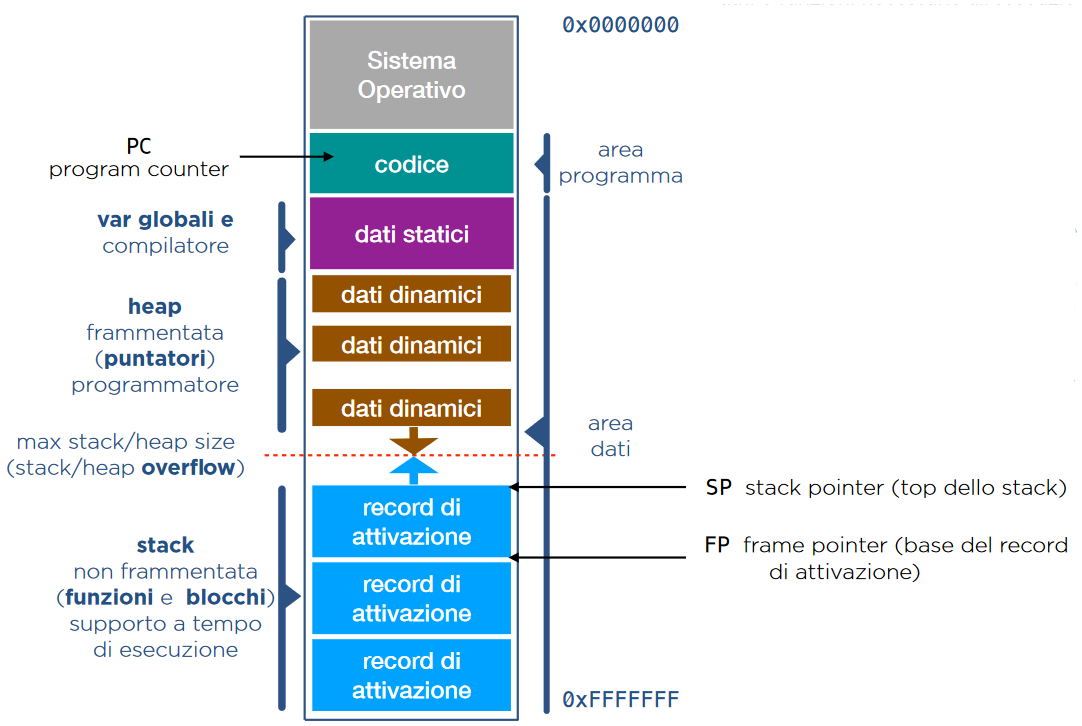
\includegraphics[width=13cm]{images/gestione-memoria.png}
	\caption{Gestione della memoria di un programma}
\end{figure}
\begin{note}
	Partiamo dal presupposto che un \textbf{blocco} sia considerato come una funzione senza parametri.
\end{note}
\begin{note}
	Lo \textbf{stack} funziona tramite operazioni di \textbf{push} (inserimento di un elemento in cima)e \textbf{pop} (rimozione dell'elemento in cima). Può lavorare in due modi:
	\begin{itemize}
		\item  \textbf{LIFO} (\emph{Last In First Out}): l'ultimo elemento inserito è il primo ad essere rimosso
		\item  \textbf{FIFO} (\emph{First In First Out}): il primo elemento inserito è il primo ad essere rimosso
	\end{itemize} 
\end{note}

\subsection{Tipi di ricorsione}
\begin{definition}[Non lineare]
	Viene eseguita più di una \textbf{chiamata ricorsiva} nel blocco. \\
	Un caso particolare è quando la funzione viene passata come parametro formale della sua stessa definizione e si dice \textbf{annidata}.
\end{definition}
\begin{definition}[Mutua]
	Quando due o più funzioni sono definite ciascuna in termini dell'altra.
\end{definition}
\begin{definition}[In coda]
	La chiamata ricorsiva è l'unica operazione effettuata dalla funzione prima di restituire il controllo alla chiamata. La chiamata in questo caso si definisce \textbf{terminale}.\\ Questa modalità consente di risparmiare spazio di memoria per la gestione dello stack di esecuzione in quando viene gestito come se fosse iterativo e viene creato un solo record di attivazione in più per la gestione dell'indirizzo di ritorno.
\end{definition}